\chapter{Model Development}\label{ch:model_development}

In this chapter several models are developed based on the simple LSTM model from the silicon-valley-data-science RNN tutorial \cite{rubashkin2017}. Firstly these models will be trained and tested on a small data set with the numbers:\\ 

$\left\{zero, one, two, three, four, five, six, seven, eight, nine \right\}$,\\\\
the same data used in Chapter \ref{ch:machine_learning} for the parameter comparison. If all the developed models achieve reasonably results, then they will be trained and tested on a bigger data set (6GB) of english speech. After that, the best performing model shall be chosen for a more detailed discription (with code).

\section{Neural Network Comparison}

Model1 (their simpleLSTM model) - pink\\
Model2 (our simpleLSTM model) - red\\
Model3 (our BiRNN model) - green

\begin{figure}[H]
	\centering
	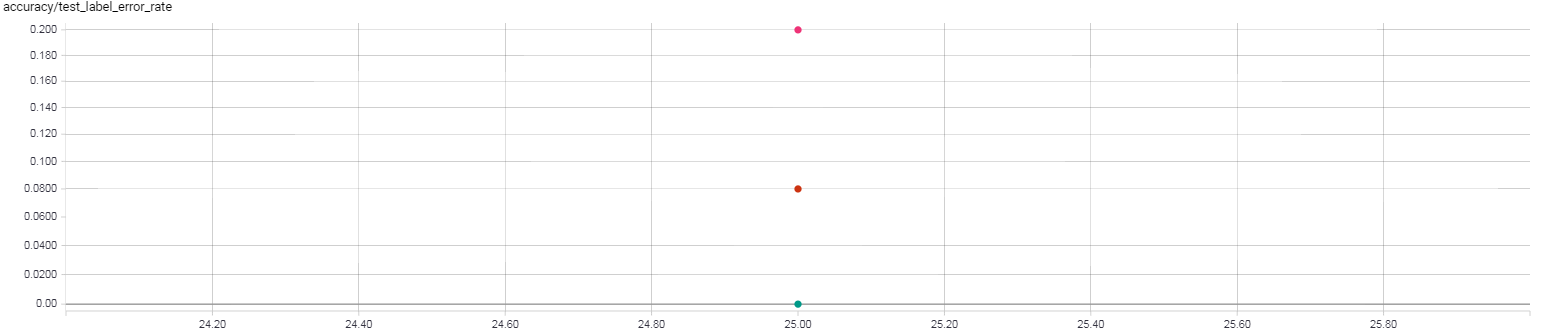
\includegraphics[width=\textwidth]		
	{model_development/3models_comparison/test_error_rate_3models}
	\caption{Test error rate.}
\end{figure}

\begin{figure}[H]
	\centering
	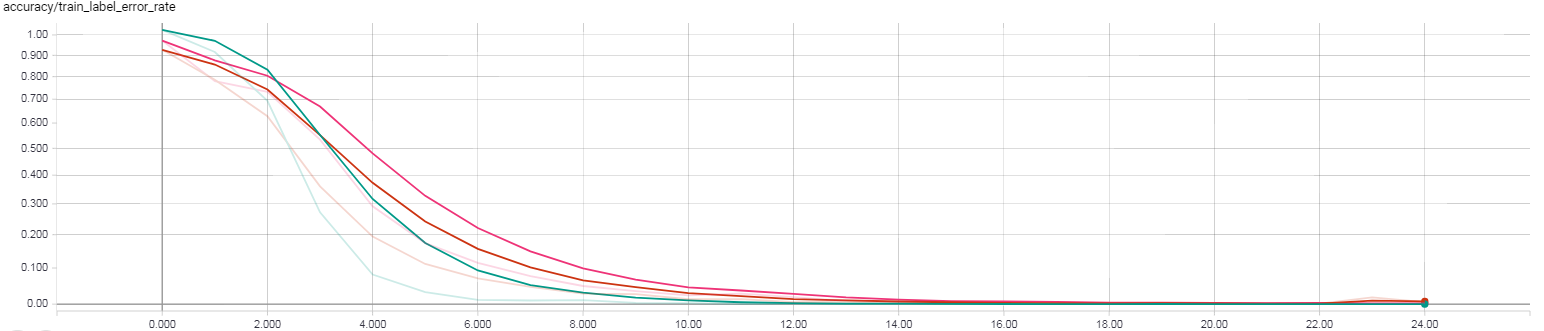
\includegraphics[width=\textwidth]		
	{model_development/3models_comparison/train_error_rate_3models}
	\caption{Training error rate.}
\end{figure}

\begin{figure}[H]
	\centering
	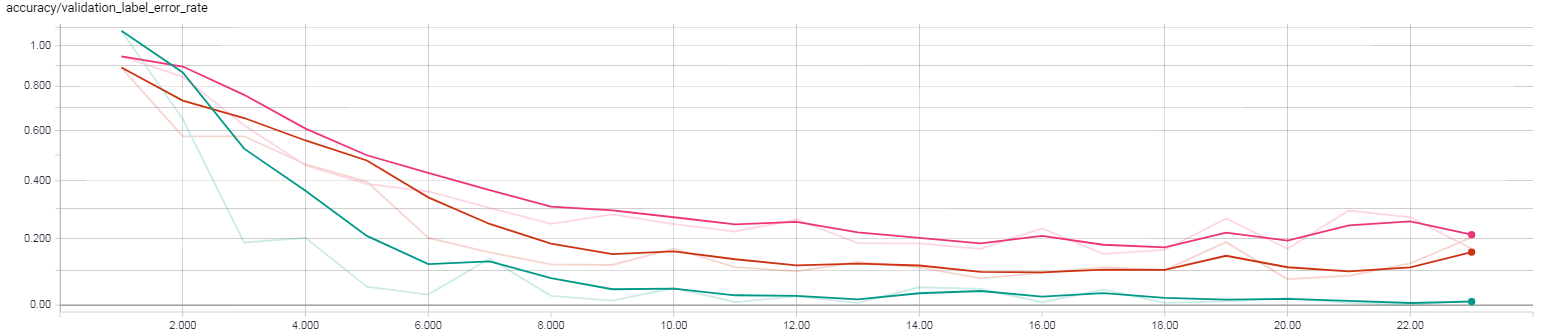
\includegraphics[width=\textwidth]		
	{model_development/3models_comparison/validation_error_rate_3models}
	\caption{Validation error rate.}
\end{figure}

\begin{figure}[H]
	\centering
	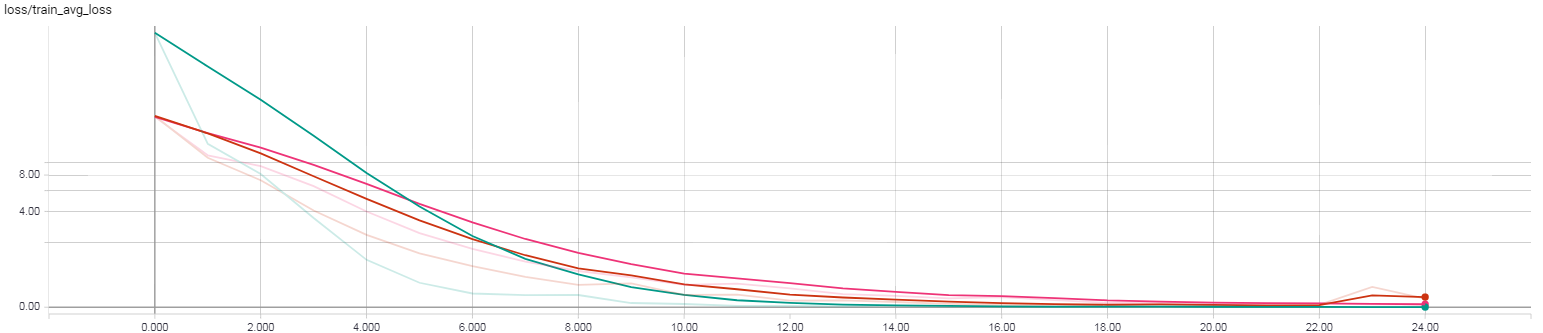
\includegraphics[width=\textwidth]		
	{model_development/3models_comparison/train_avg_loss_3models}
	\caption{Training average loss.}
\end{figure}

\section{Model Description}

Model3 (BiRNN) is better therefore we go into more detail about it...
